\chapter{Metodología de la Investigación}

\section{Diseño de la investigación}
El presente estudio emplea un diseño experimental, ya que busca evaluar el impacto de un sistema de gestión inteligente de semáforos basado en aprendizaje por refuerzo en la optimización del tráfico vehicular en la avenida Caminos del Inca, Santiago de Surco. Este diseño permite la manipulación controlada de variables, como los tiempos de luz verde y roja en los semáforos, para medir su efecto sobre indicadores clave como el tiempo de espera promedio y el flujo vehicular.
\section{Enfoque de la investigación}
El enfoque de la investigación es cuantitativo, debido a que se basa en la recopilación, análisis y modelamiento de datos numéricos obtenidos a través de fuentes digitales, como APIs de tráfico (Google Maps, Waze), y simulaciones computacionales en entornos controlados. Este enfoque asegura la objetividad y reproducibilidad de los resultados, fundamentando las conclusiones en métricas estadísticas y modelos computacionales.
\section{Alcance de la investigación}
El alcance del estudio es explicativo, ya que no solo pretende describir los patrones de tráfico existentes, sino también determinar la relación causal entre la implementación del modelo de aprendizaje por refuerzo y las mejoras en los indicadores de tráfico vehicular. Esto incluye la evaluación del desempeño del modelo en escenarios controlados y en condiciones simuladas que replican las intersecciones urbanas.
\section{Población}
La población de este estudio está constituida por la totalidad de los semáforos instalados en el distrito de Santiago de Surco, Lima. 
\section{Muestra}
La muestra seleccionada para este estudio estará compuesta por los semáforos de la avenida Caminos del Inca a distintas horas del día y durante momentos distintos de la semana.

\section{Metodología de implementación}

La metodología de esta investigación se centra en evaluar el impacto de un sistema de gestión inteligente de semáforos, basado en aprendizaje por refuerzo, aplicado a las intersecciones semaforizadas de la avenida Caminos del Inca en Santiago de Surco. Este enfoque metodológico combina un diseño experimental con técnicas de simulación computacional y análisis de datos, lo que permite establecer relaciones causales entre la implementación del modelo propuesto y las mejoras observadas en los indicadores de tráfico vehicular.

El proceso metodológico inicia con la recopilación de datos históricos y en tiempo real, obtenidos a través de APIs como Google Maps y Waze, que proporcionan información sobre densidad vehicular, tiempos de espera y patrones de tráfico. Estos datos serán complementados con herramientas de modelado y simulación como SUMO, lo que permitirá recrear las condiciones del tráfico en las intersecciones seleccionadas.

El modelo de aprendizaje por refuerzo será entrenado utilizando un marco computacional que considere las condiciones actuales de tráfico y escenarios simulados para prever su desempeño en diversas configuraciones. Las intersecciones serán tratadas como agentes autónomos dentro del sistema, capaces de ajustar dinámicamente sus fases de luz verde y roja en respuesta a las condiciones observadas.

El análisis de los resultados se centrará en indicadores clave como la reducción del tiempo promedio de espera, la disminución de la longitud de las colas vehiculares y la mejora en la fluidez del tráfico. Este enfoque permitirá no solo validar la efectividad del modelo, sino también identificar áreas de mejora para futuras implementaciones en redes de tráfico más amplias.

En la Figura \ref{metproc} se presenta de forma gráfica la metodología a seguir.

\begin{figure}[H]
    \centering
    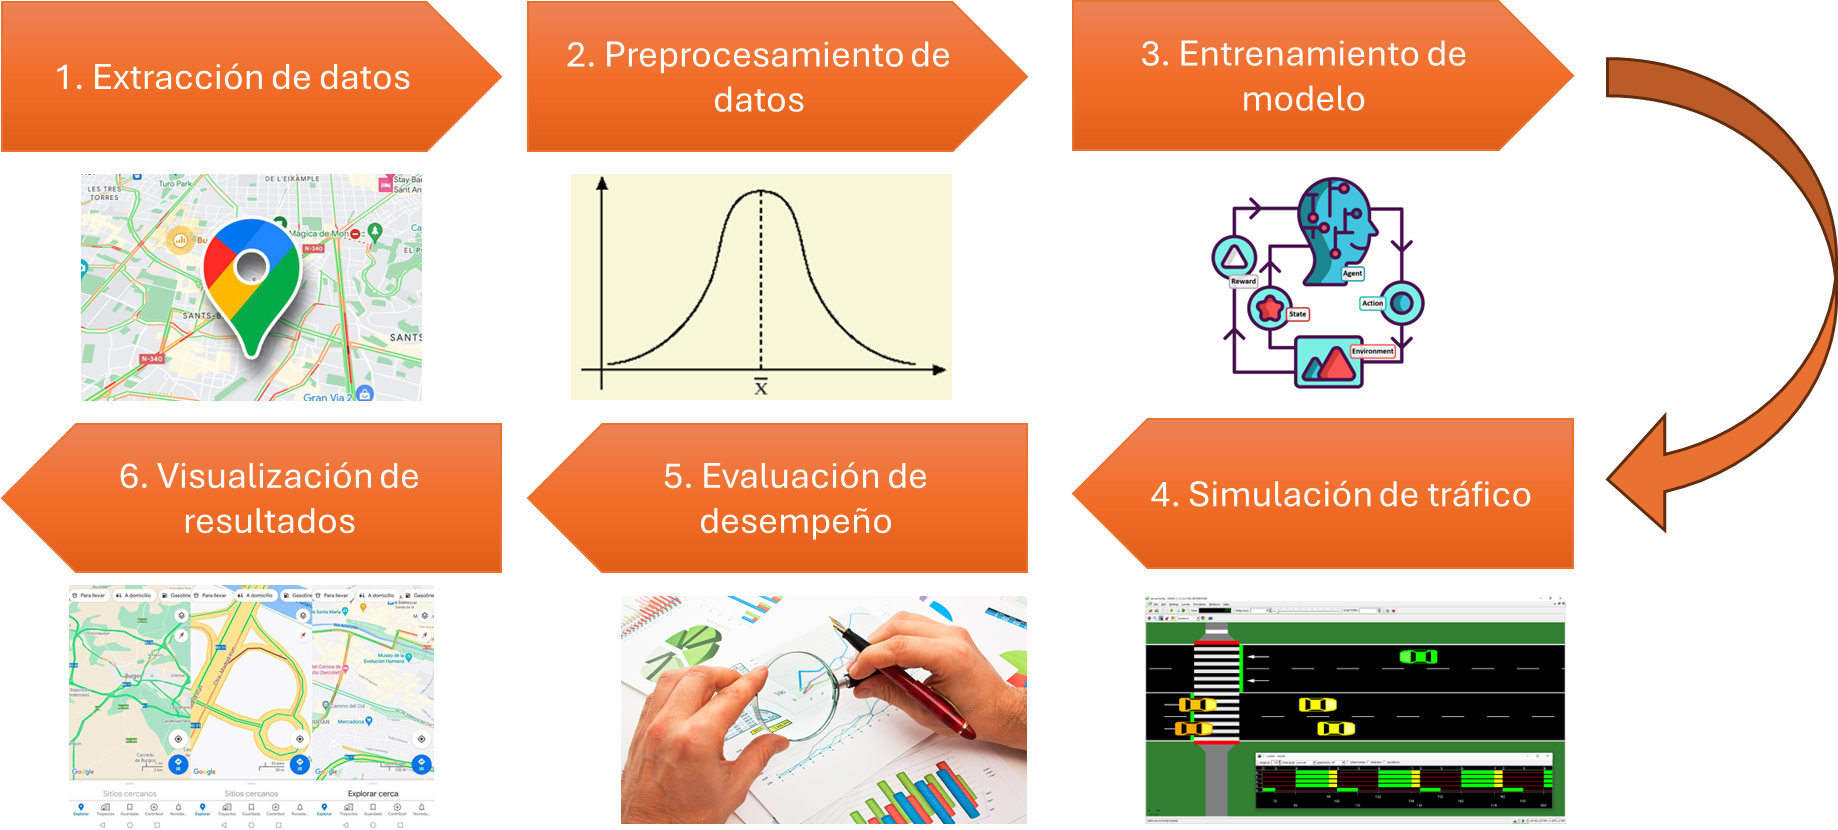
\includegraphics[width=1\linewidth]{metodologia.png}
    \caption{Metodología del proceso}
    \label{metproc}
\end{figure}

\subsection{Extracción de datos}

El primer paso de la metodología consiste en la recopilación de datos históricos y en tiempo real sobre el tráfico vehicular en las intersecciones seleccionadas de la avenida Caminos del Inca. Este proceso garantiza la obtención de información precisa y representativa para el diseño y validación del modelo de aprendizaje por refuerzo.

La recopilación de datos se llevará a cabo mediante APIs de servicios de navegación como Google Maps y Waze, que proporcionan información detallada sobre tiempos de espera, densidad vehicular y velocidades promedio en las intersecciones clave. Estos datos serán recolectados durante un período de observación de cuatro a seis semanas, abarcando tanto horas pico como no pico, para garantizar la representatividad de las diferentes condiciones de tráfico.

Además, se utilizarán herramientas de cartografía en línea como Google Maps Street View y OpenStreetMap para identificar la ubicación exacta de los semáforos en las intersecciones seleccionadas. Esta información será complementada con datos abiertos proporcionados por el municipio de Santiago de Surco, en caso de estar disponibles, para corroborar la existencia y configuración de la infraestructura semafórica.

Finalmente, se llevará a cabo un proceso de validación de los datos recolectados mediante el contraste con informes previos de tráfico y estudios de movilidad realizados en la zona. Esto asegurará que los datos utilizados sean confiables y adecuados para la simulación computacional y el entrenamiento del modelo.

\subsection{Preprocesamiento de datos}

El preprocesamiento de datos es un paso crucial para garantizar la calidad y la usabilidad de la información recolectada. Este proceso tiene como objetivo limpiar, transformar y estructurar los datos recopilados de las APIs y herramientas de navegación para que puedan ser utilizados de manera eficiente en la simulación y el entrenamiento del modelo de aprendizaje por refuerzo.

Inicialmente, los datos serán revisados para detectar inconsistencias, valores atípicos y datos faltantes. Se utilizarán técnicas de interpolación y sustitución para completar los valores ausentes y normalizar las métricas obtenidas, como los tiempos de espera, densidad vehicular y velocidades promedio. Esta normalización garantizará que los datos estén dentro de un rango uniforme, facilitando el entrenamiento del modelo.

Posteriormente, se estructurarán los datos en un formato compatible con el simulador SUMO y los algoritmos de aprendizaje por refuerzo. Esto incluye la conversión de los datos de tráfico en entradas específicas para el modelo, como estados (densidad vehicular en cada dirección), acciones (duración de las fases de semáforo) y recompensas (reducción de tiempos de espera y longitud de colas).

Finalmente, se realizará una segmentación temporal de los datos para analizar patrones de tráfico diferenciados entre horas pico y no pico. Esta segmentación permitirá entrenar el modelo bajo escenarios variados, mejorando su capacidad de generalización y adaptabilidad. Los datos procesados serán almacenados en un repositorio estructurado para su posterior uso en la etapa de simulación y modelado.

\subsection{Entrenamiento de modelo}

El entrenamiento del modelo se lleva a cabo utilizando un marco de aprendizaje por refuerzo profundo (DRL), donde cada semáforo de las intersecciones seleccionadas se representa como un agente independiente. Este agente interactúa con su entorno (condiciones de tráfico) y aprende políticas óptimas a través de un proceso iterativo de prueba y error, con el objetivo de reducir el tiempo de espera promedio y optimizar el flujo vehicular.

Para este proceso, se empleará el simulador SUMO (Simulation of Urban MObility), que permite modelar con precisión las interacciones de los vehículos y la infraestructura semafórica en escenarios urbanos. El entorno de simulación replica las condiciones de tráfico observadas en la avenida Caminos del Inca, integrando los datos procesados previamente. Este simulador proporciona un marco controlado y escalable para probar diversas configuraciones de tráfico.

El modelo se entrenará con un algoritmo de aprendizaje por refuerzo, como el Deep Q-Network (DQN), que utiliza una red neuronal profunda para aproximar las recompensas esperadas de cada acción posible. Estas acciones incluyen cambios en la duración de las fases de luz verde, amarilla y roja en cada semáforo. El entrenamiento se ejecutará en iteraciones múltiples, cada una representando un episodio en el simulador, donde el agente observa el estado del tráfico, toma decisiones y ajusta sus políticas basándose en la retroalimentación obtenida.

Durante el proceso de entrenamiento, se empleará un enfoque multiagente, permitiendo que los semáforos colaboren y compartan información para optimizar el rendimiento global del sistema de tráfico. Además, se monitorearán métricas clave como la velocidad promedio de convergencia, el tiempo de espera y la longitud de las colas vehiculares, ajustando los hiperparámetros del modelo (como la tasa de aprendizaje y el factor de descuento) para maximizar su eficiencia.

El resultado de esta etapa será un modelo entrenado capaz de operar en condiciones reales o simuladas, adaptándose dinámicamente a las variaciones del tráfico y mejorando los indicadores clave de desempeño definidos en el estudio.

\subsection{Simulación de tráfico}

La etapa de simulación de tráfico es fundamental para validar el modelo entrenado y analizar su desempeño en escenarios controlados que replican las condiciones reales de la avenida Caminos del Inca. Esta etapa se lleva a cabo utilizando el simulador SUMO (Simulation of Urban MObility), el cual permite modelar redes de tráfico urbanas con alto grado de precisión y flexibilidad.

La simulación se inicia configurando el entorno con los datos procesados previamente, incluyendo las características específicas de las intersecciones seleccionadas, como el número de carriles, las direcciones del flujo vehicular y los patrones observados en horarios pico y no pico. Asimismo, se introducen escenarios variables, como fluctuaciones en la densidad vehicular y eventos aleatorios que puedan alterar el tráfico, para evaluar la capacidad de adaptación del modelo.

El proceso de simulación se repite en múltiples episodios para obtener resultados estadísticamente significativos. Cada iteración permite ajustar los parámetros del modelo y evaluar su estabilidad y rendimiento bajo condiciones diversas. Al finalizar la simulación, se compararán los resultados obtenidos con el sistema tradicional de control fijo de semáforos, estableciendo diferencias en términos de eficiencia y reducción de congestión vehicular.

El uso de herramientas de visualización integradas en SUMO facilita la representación gráfica de los patrones de tráfico antes y después de la implementación del modelo. Estas visualizaciones son esenciales para interpretar los resultados y comunicar de manera efectiva el impacto del sistema propuesto.

\subsection{Evaluación de desempeño}

La etapa de evaluación del modelo tiene como objetivo medir el impacto del sistema de gestión inteligente de semáforos en la mejora del tráfico vehicular en las intersecciones seleccionadas. Este análisis se realiza utilizando métricas clave, las cuales permiten cuantificar la efectividad del modelo propuesto frente al sistema tradicional de control fijo.

Las métricas utilizadas son:
\begin{itemize}
    \item Tiempo promedio de espera por vehículo: Evalúa la reducción del tiempo que los vehículos permanecen detenidos en las intersecciones. Una disminución significativa en esta métrica indica una mejora en la eficiencia del flujo vehicular.
    \item Longitud promedio de las colas: Mide el nivel de congestión en las intersecciones. Esta métrica es crucial para identificar la capacidad del modelo para descongestionar puntos críticos del tráfico.
    \item Volumen vehicular procesado: Determina la cantidad de vehículos que el sistema puede gestionar en un período específico. Este indicador es esencial para evaluar la capacidad de las intersecciones bajo diferentes niveles de demanda vehicular.
\end{itemize}

La evaluación se llevará a cabo en tres etapas principales:

\begin{itemize}
    \item Comparación directa con el sistema tradicional: Se realizarán simulaciones bajo las mismas condiciones de tráfico utilizando tanto el modelo inteligente como el sistema de control fijo. Las diferencias en las métricas clave permiten cuantificar la mejora lograda.
    \item Análisis de escenarios extremos: Se evaluará el desempeño del modelo en condiciones de alta demanda vehicular (horas pico) y bajo tráfico (horas no pico). Esto asegurará que el modelo sea robusto y adaptable a diferentes contextos.
    \item Estadísticas de rendimiento agregado: Los resultados de múltiples simulaciones se promediarán para obtener valores representativos de cada métrica. Se emplean herramientas estadísticas para validar la significancia de las mejoras observadas.
\end{itemize}

\subsection{Visualización de resultados}

La visualización de resultados es una etapa clave en la metodología, ya que permite interpretar de manera clara y comprensible el impacto del modelo de gestión inteligente de semáforos sobre el tráfico vehicular. Para ello, se generarán gráficos comparativos y representaciones visuales que muestren el comportamiento del tráfico antes y después de la implementación del modelo propuesto.

Se elaborarán gráficos de barras y líneas que representen las métricas clave, como el tiempo promedio de espera, longitud de las colas y volumen vehicular procesado. Estos gráficos permitirán observar visualmente las mejoras en el flujo de tráfico bajo el nuevo sistema frente al sistema tradicional de semáforos. Por ejemplo, un gráfico de barras podría mostrar la comparación de los tiempos de espera en las intersecciones durante las horas pico antes y después de la implementación del modelo de aprendizaje por refuerzo, destacando la reducción en los tiempos de espera promedio.

Se utilizarán diagramas de dispersión y mapas de calor para visualizar la distribución del tráfico a lo largo de la avenida en diferentes horarios del día. Estos mapas facilitarán la identificación de puntos críticos y mostrarán cómo la distribución del tráfico cambia con el ajuste dinámico de los semáforos. Además, los mapas de flujo vehicular podrán ilustrar el impacto en la fluidez del tráfico en intersecciones claves, destacando las áreas con mejoras significativas en la capacidad de procesamiento de vehículos.

A través de gráficos de líneas y áreas, se podrán representar las variaciones en la longitud de las colas en tiempo real, lo que permitirá observar cómo el modelo responde a fluctuaciones en la densidad vehicular. Este tipo de visualización es crucial para entender la efectividad del sistema en escenarios de congestión extrema y su capacidad para reducir los cuellos de botella en las intersecciones.

Se desarrollarán gráficos de series temporales que muestren la evolución de los tiempos de espera y la fluidez vehicular durante las horas pico y no pico. Esto ayudará a resaltar las diferencias en el rendimiento del sistema durante diferentes períodos del día y evaluar la adaptabilidad del modelo a las variaciones en la demanda del tráfico.

Estos gráficos y representaciones serán herramientas clave no solo para la interpretación interna de los resultados, sino también para la presentación de los hallazgos a los tomadores de decisiones y otros interesados, facilitando la justificación de la efectividad del sistema propuesto.

\section{Cronograma y presupuesto}

En esta sección se observa el cronograma cumplido para el desarrollo de la primera parte de la presente tesis.

\begin{figure}[H]
    \centering
    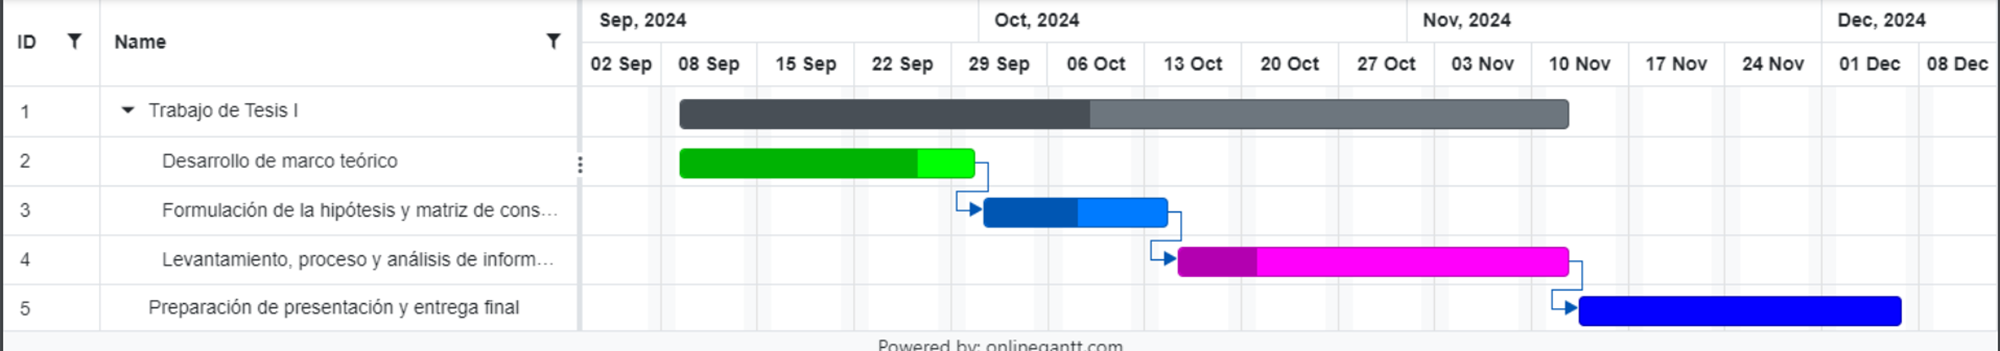
\includegraphics[width=1\linewidth]{gantt.png}
    \caption{Cronograma de primera parte}
    \label{fig:enter-label}
\end{figure}

Por otro lado, se presenta el presupuesto con los principales gastos asociados al desarrollo del modelo.

\begin{table}[H]
	\caption[Presupuesto]{Presupuesto de la investigación.}
	\label{3:table1}
	\centering
	\small
	\begin{tabular}{llll}
		\specialrule{.1em}{.05em}{.05em}
		{Grupo} & {Item} & {Costo (soles)} & {Subtotal} \\
		\specialrule{.1em}{.05em}{.05em}
	{Recursos} & {Equipo de cómputo} & {S/ 3,000.00} & {S/ 3,000.00} \\
		\cline{1-4}
        {Software} & {Simulador} & {S/ 100.00} & {} \\
		{} & {Mantenimiento de equipo} & {S/ 300.00} & {S/ 400.00} \\ % & {S/ 5,274.15} \\
		\cline{1-4}
		\multirow{2}{4cm}

	\end{tabular}
	\begin{flushleft}	
		\small Fuente: Elaboración propia.
	\end{flushleft}
\end{table}



